\RequirePackage{silence}
\documentclass[10pt,aspectratio=1610,t,xcolor={dvipsnames}]{beamer}
\usepackage{etex}
\usepackage[dvipsnames]{xcolor}
\usepackage{color, colortbl}
\usetheme[
%%% options passed to the outer them
%    hidetitle,           % hide the (short) title in the sidebar
%    hideauthor,          % hide the (short) author in the sidebar
%    hideinstitute,       % hide the (short) institute in the bottom of the sidebar
%    shownavsym,          % show the navigation symbols
%    width=2cm,           % width of the sidebar (default is 2 cm)
%    hideothersubsections,% hide all subsections but the subsections in the current section
%    hideallsubsections,  % hide all subsections
    left               % right of left position of sidebar (default is right)
%%% options passed to the color theme
%    lightheaderbg,       % use a light header background
  ]{AAUsidebar}

% If you want to change the colors of the various elements in the theme, edit and uncomment the following lines
% Change the bar and sidebar colors:
%\setbeamercolor{AAUsidebar}{fg=red!20,bg=red}
%\setbeamercolor{sidebar}{bg=red!20}
% Change the color of the structural elements:
%\setbeamercolor{structure}{fg=red}
% Change the frame title text color:
%\setbeamercolor{frametitle}{fg=blue}
% Change the normal text color background:
%\setbeamercolor{normal text}{bg=gray!10}
% ... and you can of course change a lot more - see the beamer user manual.
\WarningsOff
%%%% WARNING HACKS %%%%
%\hfuzz=\maxdimen
\hbadness=\maxdimen
\vbadness=\maxdimen
%\vfuzz=\maxdimen

\usepackage{graphicx}
\usepackage{multimedia}
\usepackage{subcaption}
\captionsetup{compatibility=false}
%\setbeamercovered{transparent}

\usepackage[utf8]{inputenc}
\usepackage[english]{babel}
\usepackage[T1]{fontenc}
% Or whatever. Note that the encoding and the font should match. If T1
% does not look nice, try deleting the line with the fontenc.
\usepackage{helvet}




% colored hyperlinks
\newcommand{\chref}[2]{%
  \href{#1}{{\usebeamercolor[bg]{AAUsidebar}#2}}%
}

\title[Agenda]% optional, use only with long paper titles
{Model Predictive Control of a Sewer System}

%\subtitle{Total fizz}  % could also be a conference name

\date{June 14, 2018}

\author[Group 1030] % optional, use only with lots of authors
{
	Group 1030 \\
  \scalebox{0.6}{Jacob Naundrup Pedersen}\\ \vspace{-1mm}
  \scalebox{0.6}{Thomas Holm Pilgaard}\\ \vspace{-1mm}
  %%\href{mailto:XX13@student.aau.dk}{{\tt mksi13@student.aau.dk}}
}
% - Give the names in the same order as they appear in the paper.
% - Use the \inst{?} command only if the authors have different
%   affiliation. See the beamer manual for an example

\institute[
%  {\includegraphics[scale=0.2]{aau_segl}}\\ %insert a company, department or university logo
  Dept.\ of Electronic Systems\\
  Aalborg University\\
  Denmark
] % optional - is placed in the bottom of the sidebar on every slide
{% is placed on the title page
  Department of Electronic Systems\\
  Aalborg University\\
  Denmark
  
  %there must be an empty line above this line - otherwise some unwanted space is added between the university and the country (I do not know why;( )
}


% specify a logo on the titlepage (you can specify additional logos an include them in 
% institute command below
\pgfdeclareimage[height=1.5cm]{titlepagelogo}{AAUgraphics/aau_logo_new} % placed on the title page
%\pgfdeclareimage[height=1.5cm]{titlepagelogo2}{graphics/aau_logo_new} % placed on the title page
\titlegraphic{% is placed on the bottom of the title page
  \pgfuseimage{titlepagelogo}
%  \hspace{1cm}\pgfuseimage{titlepagelogo2}
}

\input{Extrafeatures.tex}


\begin{document}

\usetikzlibrary{shapes,arrows}
\usetikzlibrary{plotmarks}
\pgfplotsset{compat=newest}
\pgfplotsset{filter discard warning=false}

\pgfdeclarelayer{bg}    % declare background layer
\pgfsetlayers{bg,main}


%\usepackage{silence}
%\WarningsOff[pgfplots]
%\WarningFilter{latex}{Marginpar on page}
%\WarningsOff[latex]


%%% Tikz Magic %%%
\tikzstyle{block} = [draw,rounded corners , rectangle, minimum height=3em, minimum width=6em]
\tikzstyle{Integrator} = [draw, fill=blue!20, rectangle, minimum height=5mm, minimum width=5mm]
\tikzstyle{Twolineblock} = [draw,rounded corners , rectangle, minimum height=3em, minimum width=6em, text width = 6em, align=center]     
\tikzstyle{sum} = [draw, fill=blue!20, circle, node distance=1cm]
\tikzstyle{input} = [coordinate]
\tikzstyle{output} = [coordinate]
\tikzstyle{pinstyle} = [pin edge={to-,thin,black}]
\tikzstyle{box} = [draw,rounded corners, minimum height=15mm, minimum width=20mm, align=center, text centered]
\tikzstyle{BlackBox} = [draw, fill=black, rounded corners, minimum height=15mm, minimum width=20mm, align=center, text=white, text centered]
\tikzstyle{FlowIF} = [diamond, draw, fill=blue!20, text width=8.5em, text badly centered, node distance=3cm, inner sep=0pt,align=center,aspect=3]
\tikzstyle{FlowBlock} = [rectangle, draw, fill=blue!20, text width=8em, text centered, rounded corners, minimum height=3em]
\tikzstyle{FlowCloud} = [draw, ellipse,fill=red!20, node distance=3cm, minimum height=2em]
\tikzstyle{TestBox} = [rectangle,draw, fill=black!20, minimum height=8mm, minimum width=8mm]
\tikzstyle{TestDiamond} = [diamond, draw, fill=black!20, minimum height=10.5mm, minimum width=10.5mm]
\tikzstyle{TestBox} = [rectangle,draw, fill=black!20, minimum height=8mm, minimum width=8mm]
\tikzstyle{TestCircle} = [circle, draw, fill=black!20, minimum height=6mm, minimum width=6mm]
\tikzstyle{TestTable} = [rectangle, draw, fill=black!60, minimum height=0.01mm, minimum width=9mm, text=white]
\tikzstyle{TestBoxSmall} = [rectangle,draw, fill=black!, minimum height=8mm, minimum width=8mm,text=white]
\tikzstyle{LegendBox} = [rectangle,draw, minimum height=7mm, minimum width=20mm]
\tikzstyle{Sysbox} = [draw,rounded corners, minimum height=15mm, minimum width=9em, align=center, text centered,text width = 10.5em]
\tikzstyle{SysBlackBox} = [draw, fill=black, text=white, rounded corners, minimum height=15mm, minimum width=9em, align=center, text centered,text width = 10em]
\tikzstyle{PreAmpBox} = [rectangle,draw, fill=black!20, minimum height=8mm, minimum width=12mm]
\tikzstyle{gain} = [fill=white, draw, rectangle, minimum height=2.5em, minimum width=2.5em]
\tikzstyle{summation} = [draw, minimum size=0.75cm, circle, node distance=1.75cm]












%% Its a pie chart!! %%%
\definecolor{rosso}{RGB}{220,57,18}
\definecolor{giallo}{RGB}{255,153,0}
\definecolor{blu}{RGB}{102,140,217}
\definecolor{verde}{RGB}{16,150,24}
\definecolor{viola}{RGB}{153,0,153}

\makeatletter

\tikzstyle{chart}=[
    legend label/.style={font={\scriptsize},anchor=west,align=left},
    legend box/.style={rectangle, draw, minimum size=5pt},
    axis/.style={black,semithick,->},
    axis label/.style={anchor=east,font={\tiny}},
]

\tikzstyle{bar chart}=[
    chart,
    bar width/.code={
        \pgfmathparse{##1/2}
        \global\let\bar@w\pgfmathresult
    },
    bar/.style={very thick, draw=white},
    bar label/.style={font={\bf\small},anchor=north},
    bar value/.style={font={\footnotesize}},
    bar width=.75,
]

\tikzstyle{pie chart}=[
    chart,
    slice/.style={line cap=round, line join=round, very thick,draw=white},
    pie title/.style={font={\bf}},
    slice type/.style 2 args={
        ##1/.style={fill=##2},
        values of ##1/.style={}
    }
]

\pgfdeclarelayer{background}
\pgfdeclarelayer{foreground}
\pgfsetlayers{background,main,foreground}



\newcommand{\pie}[3][]{
    \begin{scope}[#1]
    \pgfmathsetmacro{\curA}{90}
    \pgfmathsetmacro{\r}{1}
    \def\c{(0,0)}
    \node[pie title] at (90:1.3) {#2};
    \foreach \v/\s in{#3}{
        \pgfmathsetmacro{\deltaA}{\v/100*360}
        \pgfmathsetmacro{\nextA}{\curA + \deltaA}
        \pgfmathsetmacro{\midA}{(\curA+\nextA)/2}

        \path[slice,\s] \c
            -- +(\curA:\r)
            arc (\curA:\nextA:\r)
            -- cycle;
        \pgfmathsetmacro{\d}{max((\deltaA * -(.5/50) + 1) , .5)}

        \begin{pgfonlayer}{foreground}
        \path \c -- node[pos=\d,pie values,values of \s]{$\v\%$} +(\midA:\r);
        \end{pgfonlayer}

        \global\let\curA\nextA
    }
    \end{scope}
}




%% Cutom legned entry
\newenvironment{customlegend}[1][]{%
	\begingroup
	% inits/clears the lists (which might be populated from previous
	% axes):
	\csname pgfplots@init@cleared@structures\endcsname
	\pgfplotsset{#1}%
}{%
% draws the legend:
\csname pgfplots@createlegend\endcsname
\endgroup
}%

% makes \addlegendimage available (typically only available within an
% axis environment):
\def\addlegendimage{\csname pgfplots@addlegendimage\endcsname}

\usetikzlibrary{arrows}
\tikzset{>=stealth}


%% Its Color time:
\definecolor{MATLABblue}{rgb}{0,0.4470,0.7410}
\definecolor{MATLABorange}{rgb}{0.85,0.3250,0.0980}
\definecolor{MATLAByellow}{rgb}{0.929,0.6940,0.1250}
\definecolor{MATLABpurple}{rgb}{0.494,0.1840,0.5560}
\definecolor{MATLABgreen}{rgb}{0.466,0.6740,0.1880}
\definecolor{MATLABbabyblue}{rgb}{0.301,0.7450,0.9330}
\definecolor{MATLABred}{rgb}{0.635,0.0780,0.1840}
%% Loopback color
\definecolor{MATLABblack}{rgb}{0,0,0}

%% Microphone Colors
\definecolor{M1}{rgb}{0,0.4470,0.7410}
\definecolor{M2}{rgb}{0.85,0.3250,0.0980}
\definecolor{M3}{rgb}{0.929,0.6940,0.1250}
\definecolor{M4}{rgb}{0.494,0.1840,0.5560}
\definecolor{M5}{rgb}{0.466,0.6740,0.1880}
\definecolor{M6}{rgb}{0.301,0.7450,0.9330}
\definecolor{M7}{rgb}{0.635,0.0780,0.1840}
\definecolor{M8}{rgb}{0,0,1}
\definecolor{M9}{rgb}{0,0.5,1}
\definecolor{M10}{rgb}{0,1,0.5}
\definecolor{M11}{rgb}{0,1,1}
\definecolor{M12}{rgb}{0.5,1,0.5}
\definecolor{M13}{rgb}{1,0.5,0}
\definecolor{M14}{rgb}{1,0,0}
\definecolor{M15}{rgb}{0.5,0,0}

\newcommand*\circled[1]{\tikz[baseline=(char.base)]{
		\node[shape=circle,draw,inner sep=2pt] (char) {#1};}}



\newenvironment{sbmatrix}[1]
{\def\mysubscript{#1}\mathop\bgroup\begin{bmatrix}}
	{\end{bmatrix}\egroup_{\textstyle\mathstrut\mysubscript}}

\usetikzlibrary{matrix,calc}
\tikzstyle{loosely dotted}=[dash pattern=on 2\pgflinewidth off 24pt]

% \makeatletter
% \renewcommand{\todo}[2][]{\tikzexternaldisable\@todo[#1]{#2}\tikzexternalenable}
% \makeatother

% %\makeatletter
% %\renewcommand{\missingfigure}[2][]{\tikzexternaldisable\@missingfigure[#1]{#2}\tikzexternalenable}
% %\makeatother

% \let\oldmissingfigure\missingfigure
% \renewcommand{\missingfigure}[2][]{\tikzexternaldisable\oldmissingfigure[#1]{#2}\tikzexternalenable}
% the titlepage
{\aauwavesbg%
\begin{frame}[plain,noframenumbering] % the plain option removes the sidebar and header from the title page
  \titlepage
\end{frame}}
%%%%%%%%%%%%%%%%

% TOC
\begin{frame}{Agenda}{}
\tableofcontents
\end{frame}

%%%%%%%%%%%%%%%%


\section{Control}
%%%%%%%%%%%% MID WAY AGENDA %%%%%%%%%%%%%%
%\begin{frame}<beamer>
%\frametitle{Simon Bjerre Krogh}
%\tableofcontents[currentsection]
%\end{frame}


% the license


\begin{frame}{Controller}{}

\begin{figure}[H]
\centering


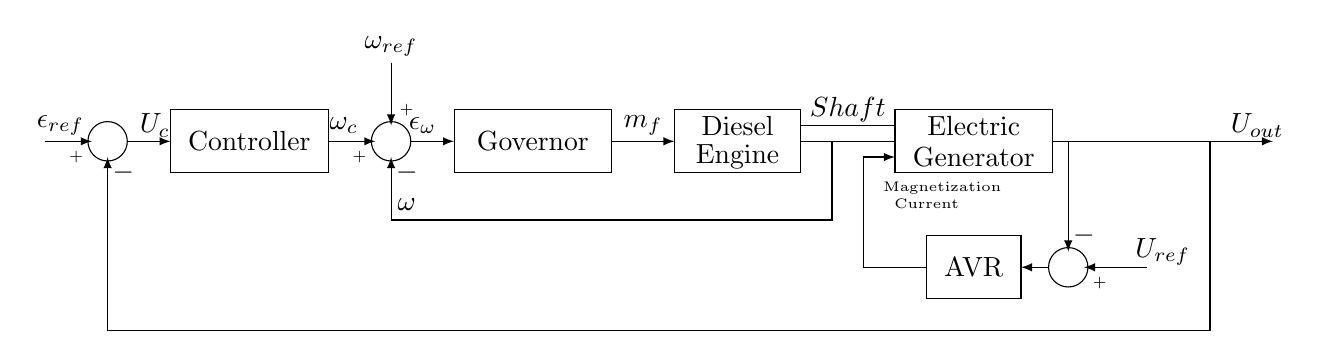
\begin{tikzpicture}

 \node at (2,0.2) {\normalsize{Governor}};
\draw [-latex] (1,0.6) rectangle (3,-0.2);
 \node at (4.6,0.4) {\normalsize{Diesel}};
  \node at (4.6,0) {\normalsize{Engine}};
\draw [-latex] (3.8,0.6) rectangle (5.4,-0.2);
\draw [-latex](3,0.2) -- (3.8,0.2);
\node at (3.4,0.4) {$m_f$};
 \node at (7.6,0.4) {\normalsize{Electric}};
  \node at (7.6,0) {\normalsize{Generator}};
\draw [-latex] (6.6,0.6) rectangle (8.6,-0.2);

\node at (6,0.6) {$Shaft$};
  \node at (7.6,-1.4) {\normalsize{AVR}};
\draw [-latex] (8.8,-1.4) ellipse (0.25 and 0.25);
\draw [-latex] (7,-1) rectangle (8.2,-1.8);
\draw [-latex](7,-1.4) -- (6.2,-1.4) -- (6.2,0) -- (6.6,0);
\node at (9,-1) {$-$};
\draw [-latex](9.8,-1.4) -- (9,-1.4);
\node at (10,-1.2) {$U_{ref}$};
\node at (7.2,-0.4) {\tiny{Magnetization}};
\node at (7,-0.6) {\tiny{Current}};
\node at (11.2,0.4) {$U_{out}$};
\draw [-latex] (0.2,0.2) ellipse (0.25 and 0.25);

\draw [-latex](0.2,1.2) -- (0.2,0.4);
\node at (0.2,1.4) {$\omega_{ref}$};
\draw [-latex](5.8,0.2) -- (5.8,-0.8) -- (0.2,-0.8) -- (0.2,0);
\node at (0.4,-0.6) {$\omega$};
\node at (-1.6,0.2) {\normalsize{Controller}};
\draw [-latex] (-2.6,0.6) rectangle (-0.6,-0.2);
\draw [-latex](-0.6,0.2) -- (0,0.2);
\node at (-0.4,0.4) {$\omega_{c}$};
\draw [-latex] (-3.4,0.2) ellipse (0.25 and 0.25);
\draw [-latex](-3.15,0.2) -- (-2.6,0.2);
\node at (-2.8,0.4) {$U_{c}$};
\draw [-latex](-4.2,0.2) -- (-3.6,0.2);
\node at (-4,0.4) {$\epsilon_{ref}$};
\draw [-latex](10.6,0.2) -- (10.6,-2.2) -- (-3.4,-2.2) -- (-3.4,0);
\node at (-3.2,-0.2) {$-$};
\node at (0.6,0.4) {$\epsilon_{\omega}$};
\draw [-latex](8.8,0.2) -- (8.8,-1.2);
\draw [-latex](8.6,0.2) -- (11.4,0.2);
\draw [-latex](8.55,-1.4) -- (8.2,-1.4);
\draw [thin](5.4,0.2) -- (6.6,0.2);
\draw [thin](5.4,0.4) -- (6.6,0.4);
\draw [thin](0.4,0.2);
\draw [-latex](0.45,0.2) -- (1,0.2);
\node at (-3.8,0) {\tiny{+}};





\node at (9.2,-1.6) {\tiny{+}};
\node at (0.4,-0.2) {$-$};
\node at (0.4,0.6) {\tiny{+}};
\node at (-0.2,0) {\tiny{+}};

\end{tikzpicture} 
\caption{ Block diagram illustrating the genset with an added controller.}
\end{figure}

\end{frame}


\begin{frame}{Controller}{}
\begin{figure}[H]
\centering
\subsection{Disturbances affecting the system}
\label{disturbances}

In \secref{statespace_disturbance}, the two kinds of disturbances were introduced, namely the load and the inverter. The inverter, as it was mentioned, provides a slowly changing power flow that can be approximated as a sinusoidal shown in \eqref{eq:dist1} : 

\begin{equation}
  \label{eq:dist1}
    d_{inv}(t) = \alpha sin(\omega t)
  \end{equation}

By solving \eqref{eq:ss_tf1} and \eqref{eq:ss_tf2} the state space system can be constructed: 


\begin{equation}
\label{eq:exo_statespace}
 \begin{bmatrix}
    \dot{x}_{d1} \\
    \dot{x}_{d2}
\end{bmatrix}
=
 \begin{bmatrix}
    0 & \omega^2 \\
    -\omega^2 & 0
\end{bmatrix}
 \begin{bmatrix}
    x_{d1} \\
    x_{d2}
\end{bmatrix}
\end{equation}

\begin{equation}
\label{eq:ss_dist2}
    d
=
 \begin{bmatrix}
    1 & 0 
\end{bmatrix}
 \begin{bmatrix}
    x_{d1} \\
    x_{d2}
\end{bmatrix}
\end{equation}

The characteristic polynomial of the sinusoidal disturbance system, as expected is: 

\begin{equation}
  \label{eq:distpoly}
    \Gamma_{inverter}(s) = det(s\mathbf{I}-\mathbf{A_d}) = s^2 + \omega^2 
  \end{equation}
  
%The case of the load however is significantly different from the case of the inverter. The load is, as mentioned, usually unknown and can produce big changes. The fact that the behaviour of the load is completely unknown in reality cannot be neglected, however in the simulation a constant load is described to show how the system can reject it. The reason behind making a disturbance that dramatically affects the voltage output of the system is that if the load was constant, a slowly varying inverter power flow would never cause changes on the output. That is because the AVR and the other inner controllers can easily handle slow disturbances such as the inverter power flow. 


In order to construct the combination of the two disturbances, the following rule applies: 

\begin{equation}
  \label{eq:combined_dist}
  d(t) = d_{inv}(t) + d_{load}(t) = \Gamma_{inv}(s)\Gamma_{load}(s)
  \end{equation}
  
As can be seen in \eqref{eq:combined_dist}, the combined disturbance system can be calculated by multiplying the disturbance generating polynomials for $d_{inv}(t)$ and $d_{load}(t)$. Thus, the final form of the disturbance becomes: 

\begin{equation}
  \label{eq:dist_final}
  d(t) = d_{inv}(t) + d_{load}(t) = c + \alpha sin(\omega t)
  \end{equation}

that is a slowly-varying sinusoidal disturbance with an offset.  
\caption{}
\end{figure}

\end{frame}




\begin{frame}{Controller}{}

\begin{figure}[H]
\centering
\input{Tikz/controlstructure.tex} 
\caption{}
\end{figure}


\end{frame}

%%%%%%%%%%%%%%%%
\section{Results}
%%%%%%%%%%%% MID WAY AGENDA %%%%%%%%%%%%%%
%\begin{frame}<beamer>
%\frametitle{Thomas Holm Pilgaard}
%\tableofcontents[currentsection]
%\end{frame}
%%%%%%%%%%%% MID WAY AGENDA %%%%%%%%%%%%%%

\begin{frame}{Controller}{}

\begin{figure}[H]
\centering
\input{Tikz/estimation.tex} 
\caption{Figure illustrating the output without and with controller at a scaling factor K=0.1.}
\end{figure}

\end{frame}

\begin{frame}{Introduction}{}

\begin{figure}[H]
\centering
\includegraphics[width=1\textwidth]{Sections/Billeder/result_1020_4050}
%\caption{Picture of genset and SMA STP25000 inverter (yellow box)}
\end{figure}


\end{frame}



\begin{frame}{Introduction}{}

\begin{figure}[H]
\centering
\includegraphics[width=1\textwidth]{Sections/Billeder/result_1030_1050}
%\caption{Picture of genset and SMA STP25000 inverter (yellow box)}
\end{figure}


\end{frame}



\end{document}
